\documentclass[UTF8]{ctexart}
\usepackage{geometry}
\usepackage[backend=biber, style=authoryear]{biblatex} % 示例配置
\addbibresource{references.bib} % 替换为你的参考文献文件
\geometry{margin=1.5cm, vmargin={0pt,1cm}}
\setlength{\topmargin}{-1cm}
\setlength{\paperheight}{29.7cm}
\setlength{\textheight}{25.3cm}

% useful packages.
\usepackage{amsfonts}
\usepackage{amsmath}
\usepackage{amssymb}
\usepackage{amsthm}
\usepackage{enumerate}
\usepackage{graphicx}
\usepackage{multicol}
\usepackage{fancyhdr}
\usepackage{layout}
\usepackage{listings}
\usepackage{xcolor}
\usepackage{multirow}
\lstset{language=C++}
\setlength{\headheight}{13pt}  % 增加头部高度
\usepackage{float, caption}

% Listings setting for code formatting
\lstset{
    basicstyle=\ttfamily,
    keywordstyle=\color{blue},
    commentstyle=\color{gray},
    stringstyle=\color{red},
    breaklines=true,
    frame=single,
    numbers=left,
    numberstyle=\tiny,
    stepnumber=1,
    tabsize=4
}

% some common commands
\newcommand{\dif}{\mathrm{d}}
\newcommand{\avg}[1]{\left\langle #1 \right\rangle}
\newcommand{\difFrac}[2]{\frac{\dif #1}{\dif #2}}
\newcommand{\pdfFrac}[2]{\frac{\partial #1}{\partial #2}}
\newcommand{\OFL}{\mathrm{OFL}}
\newcommand{\UFL}{\mathrm{UFL}}
\newcommand{\fl}{\mathrm{fl}}
\newcommand{\op}{\odot}
\newcommand{\Eabs}{E_{\mathrm{abs}}}
\newcommand{\Erel}{E_{\mathrm{rel}}}

\begin{document}

\pagestyle{fancy}
\fancyhead{}
\lhead{陈梓锐}
\chead{22435036}
\rhead{\today}


%\begin{abstract}
 %   The abstract is not necessary for the theoretical homework, 
   % but for the programming project, 
    %you are encouraged to write one.      
%\end{abstract}

% ============================================
\subsection*{如何使用}
在code中build文件下使用make命令编译，编译成功后，在build文件夹下会生成可执行文件main,在test目录下的main.json调整初始条件即可使用不同的测试用例。

在文件EquationSolverFactory.h中，设计了工厂模式以及单例模式，为选择不同的求解器提供了方便。

\begin{lstlisting}[language=C++]
{
    "FuncName" : "Func",
    "method" : "AB4",
    "output_file" : "output",
    "condition_type" : 1,
    "step" :200000,
    "print_accurate" : false,
    "is_test" : false
}
\end{lstlisting}

\begin{enumerate}
    \item method选择不同的方法与精度
    \item conditiontype选择不同的初始条件
    \item step选择不同的步长
    \item print\_accurate选择是否打印数值精度
    \item is\_test选择是否进行测试
\end{enumerate}


\subsection*{CRK方法在步长6000}
\begin{figure}[H]
    \centering
    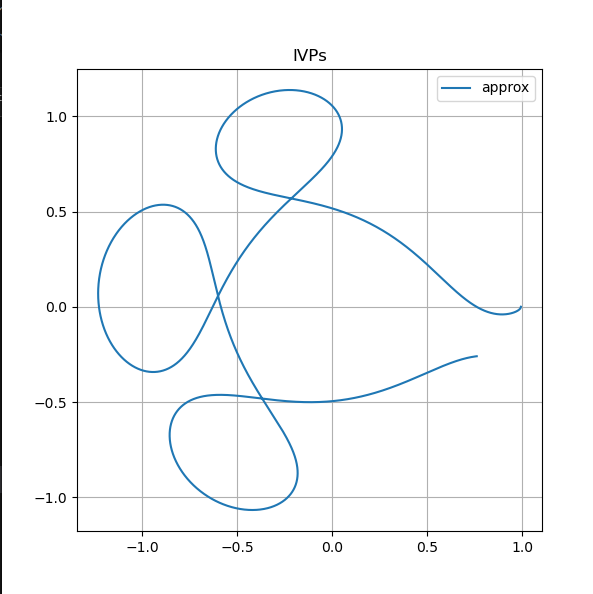
\includegraphics[width=0.3\textwidth]{CRK1.png}
    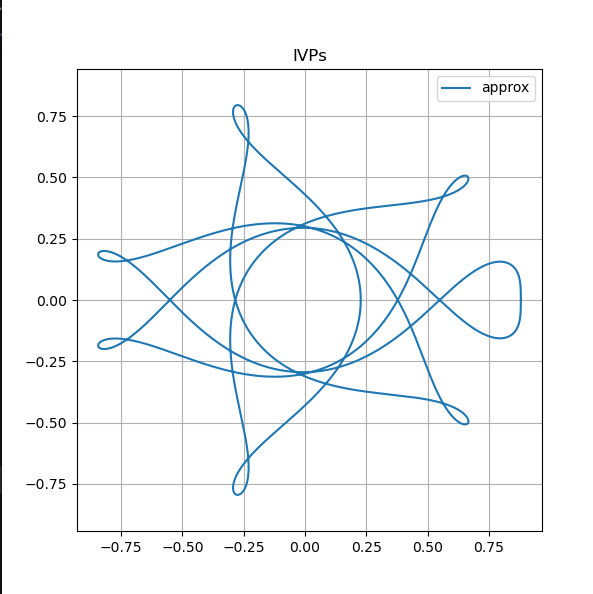
\includegraphics[width=0.3\textwidth]{CRK2.png}
    \caption{CRK方法}
\end{figure}
注意到CRK方法在6000步时图像与真实值有较大差异，是因为步长过大导致的，
只要减小步长，就可以得到比较好的结果。
\begin{enumerate}
    \item [CRK] 误差 = 2.15143, 
    Total CPU Time : 0.033 seconds.
    
    \item [CRK] 误差 = 9.8895e-08, 
    Total CPU Time : 0.061 seconds.
    
\end{enumerate}

\subsection*{ESDIRK方法在步长24000}
\begin{figure}[H]
    \centering
    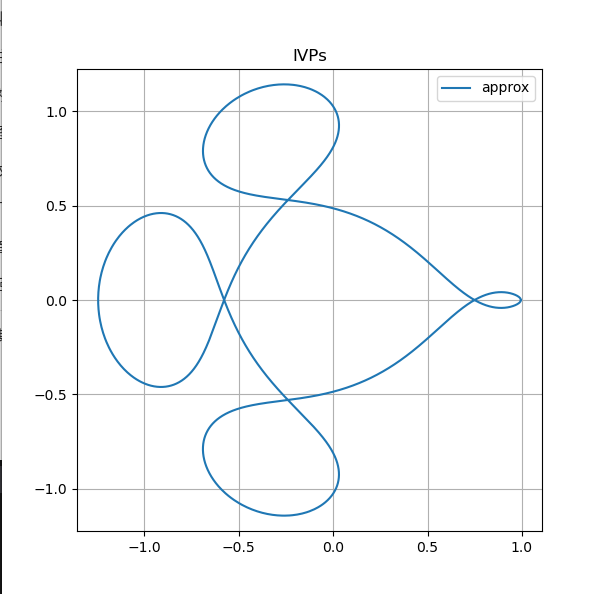
\includegraphics[width=0.3\textwidth]{ESDIRK1.png}
    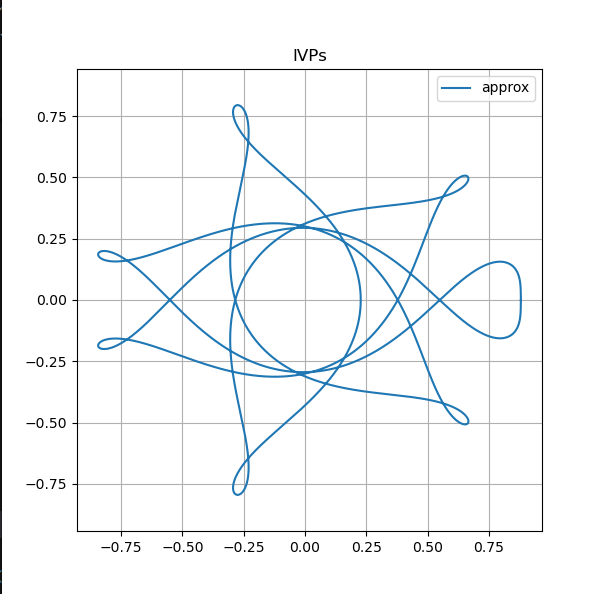
\includegraphics[width=0.3\textwidth]{ESDIRK2.png}
    \caption{ESDIRK方法}
\end{figure}
\begin{enumerate}
    \item [ESDIRK] 误差 = 0.0608162, 
    Total CPU Time : 5.519 seconds.
    \item [ESDIRK] 误差 = 1.06391e-11, 
    Total CPU Time : 5.822 seconds.
\end{enumerate}

\subsection*{Feldberg方法在步长100}
\begin{figure}[H]
    \centering
    
\includegraphics[width=0.3\textwidth]{F1.png}
    
\includegraphics[width=0.3\textwidth]{F2.png}
    \caption{Feldberg方法}
\end{figure}
\begin{enumerate}
    \item [Fehlberg method] 误差 = 1.95975, 
    Total CPU Time : 0.016 seconds.
    \item [Fehlberg method] 误差 = 0.170646, 
    Total CPU Time : 0.017 seconds.
\end{enumerate}

\subsubsection*{Dormand-Prince方法在步长100}
\begin{figure}[H]
    \centering
    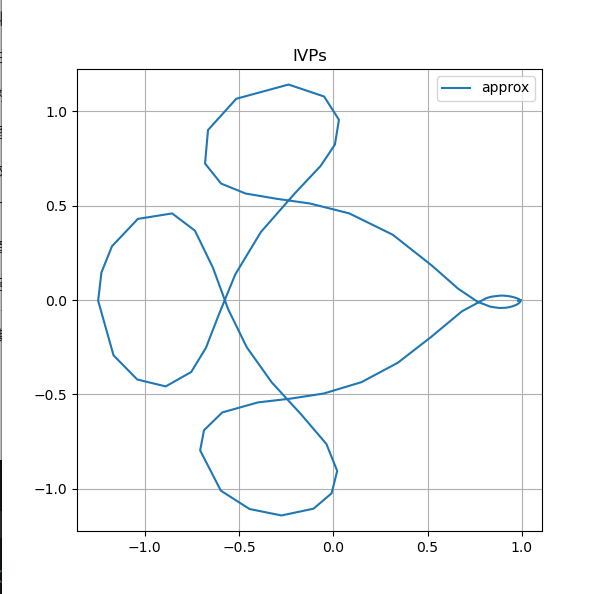
\includegraphics[width=0.3\textwidth]{DP1.png}
    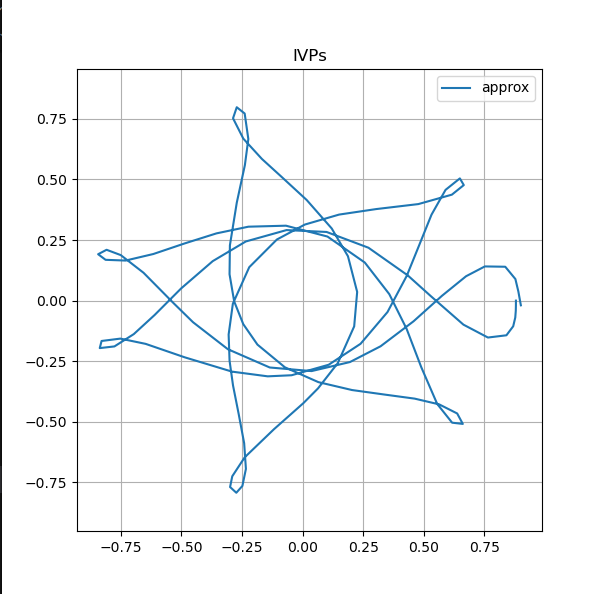
\includegraphics[width=0.3\textwidth]{DP2.png}
    \caption{Dormand-Prince方法}
\end{figure}
\begin{enumerate}
    \item [Dormand-Prince method] 误差 = 2.41591, 
    Total CPU Time : 0.02 seconds.    
    \item [Dormand-Prince method] 误差 = 0.104859, 
    Total CPU Time : 0.006 seconds.
\end{enumerate}




\subsection*{收敛阶}
对于一个p阶方法，用步长h求解一个IVPs时，其全局误差E(h)应满足$E(h)\approx O(h^{p})$。
对于两个不同的网格$h_1=\frac{T}{N_1}, h_2=\frac{T}{N_2}$,可以用式$p\approx \frac{log(E_1/E_2)}{log(h_1/h_2)}$来估算收敛阶。

下面我们利用（10.93）式，计算收敛阶。

\begin{table}[H]
    \centering
    \caption{AB4、BDF4 与 AM5 方法在不同步长下的误差与收敛阶}
    \begin{tabular}{|c|c|c|c|c|}
    \hline
    方法 & $N$ & 步长 $h$ & 误差 $\|u - u_h\|$ & 收敛阶 $p$ \\
    \hline
    \multirow{4}{*}{AB4}
    & 10000 & 0.00191405  & $2.20725 \times 10^{-6}$ & --     \\
    & 20000 & 0.00095703  & $7.80855 \times 10^{-8}$ & 4.82   \\
    & 40000 & 0.00047851  & $9.30889 \times 10^{-9}$ & 3.07   \\
    & 80000 & 0.00023926  & $6.64014 \times 10^{-10}$ & 3.81  \\
    \hline
    \multirow{4}{*}{BDF4}
    & 10000 & 0.00191405  & $1.48016 \times 10^{-6}$ & --     \\
    & 20000 & 0.00095703  & $4.05638 \times 10^{-8}$ & 5.19   \\
    & 40000 & 0.00047851  & $5.26787 \times 10^{-9}$ & 2.94   \\
    & 80000 & 0.00023926  & $5.22306 \times 10^{-10}$ & 3.33  \\
    \hline
    \multirow{4}{*}{AM5}
    & 10000 & 0.00191405  & $1.93293 \times 10^{-7}$ & --     \\
    & 20000 & 0.00095703  & $6.11855 \times 10^{-9}$ & 4.98   \\
    & 40000 & 0.00047851  & $2.64776 \times 10^{-10}$ & 4.53  \\
    & 80000 & 0.00023926  & $9.28519 \times 10^{-11}$ & 1.51  \\
    \hline
    \end{tabular}
\end{table}

发现AB4和BDF4的收敛阶都超过了4,这是因为初值给定的非常精确而出现了超收敛的现象。

而AM5的收敛阶却突然减小，原因是其误差已经达到了机器精度，导致相对误差变得不再可靠。

% ===============================================

\end{document}